\documentclass{article}

% Language setting
% Replace `english' with e.g. `spanish' to change the document language
\usepackage[russian]{babel}
\usepackage{amsmath}

%графика
\usepackage{wrapfig}
\usepackage{graphicx}
\usepackage{pgfplots}
\usepackage{tikz}


\usepackage{tcolorbox}

% Set page size and margins
% Replace `letterpaper' with `a4paper' for UK/EU standard size
\usepackage[letterpaper,top=2cm,bottom=2cm,left=3cm,right=3cm,marginparwidth=1.75cm]{geometry}

% Useful packages
\usepackage{amsmath}
\usepackage{amssymb}
\usepackage{graphicx}
\usepackage{fixltx2e}
\usepackage[colorlinks=true, allcolors=blue]{hyperref}
\usepackage{subcaption}
\usepackage{caption}

\usepackage{hyperref}

\usepackage{makecell}
\renewcommand\theadalign{bc}
\renewcommand\theadfont{\bfseries}
\renewcommand\theadgape{\Gape[4pt]}
\renewcommand\cellgape{\Gape[4pt]}

\usepackage{geometry}
\geometry{left=25mm,right=25mm,
	top=25mm,bottom=25mm}

\newcommand{\specialcell} [2] [c] { {% 
		\def\arraystretch{2}%
		\begin{tabular} [#1] {@{}c@{}} #2 \end{tabular}}}

\title{Quantitative Analytics.\\
	Lectures. Week 5. \\
	Introduction to Industry And Company Analysis. Введение в анализ компаний и индустрии.}
\author{Akhundzhanova Elina}

% Колонтитулы
\usepackage{fancyhdr}
\pagestyle{fancy}
\renewcommand{\headrulewidth}{0.1mm}  
\renewcommand{\footrulewidth}{0.1mm}
\lfoot{}
\rfoot{\thepage}
\cfoot{}
\rhead{CMF-2022}
\chead{}
%\renewcommand{\figurename}{Рис.}

\begin{document}
	\maketitle
	
	% Оглавление
	\setcounter{tocdepth}{2} % - в оглавлении участвуют chapter, section и subsection. {1} - только chapter и section
	\renewcommand\contentsname{Содержание}
	\tableofcontents
	\newpage
	
	% \section{Dictionary, Definitions, Abbreviations}
	
	% \subsection{Dictionary}
	% \begin{itemize}
		%     \item IR - Interest rate - процентная ставка.
		%     \item Compounding - платежи (idk)
		% \end{itemize}
	
	% \subsection{Definitions and Abbreviations}
	% \begin{itemize}
		%     \item SAR - Stated annual rate.
		%     \item EAR - Effective annual rate.
		%     \item FoC - Frequency of Compounding
		%     \item PMT - Payment
		%     \item r - Interest rate (at the moment). 
		% \end{itemize}
	
	\renewcommand{\labelitemi}{\tiny$\bullet$}
	\renewcommand{\figurename}{Рис.}
	
	\section{Для чего нужен анализ секторов экономики и индустрий?}
	\begin{enumerate}
		\item \textbf{Анализ секторов экономики и индустрий помогает разобраться в деятельности компании, акции которой мы хотим оценить.} Так как компании не существуют в вакууме, они работают в конкуретной среде, то практически для каждой компании всегда найдется конкурент, работающий на том же рынке. Лучше разобравшись в том, как устроена та или иная отрасль экономики, мы начнем гораздо лучше понимать саму компанию и сможем гораздо точнее оценить перспективы ее акций.
		
		\item \textbf{Для активного управления портфелем}. То есть мы меняем портфель в зависимости от того, в какой стадии экономического цикла сейчас находится экономика. Ниже приведена таблица, в которой показано, как ведут себя акции различных секторов в ранней, средней, поздней стадиях и стадии рецессии.
		\begin{figure}[h]
			\centering
			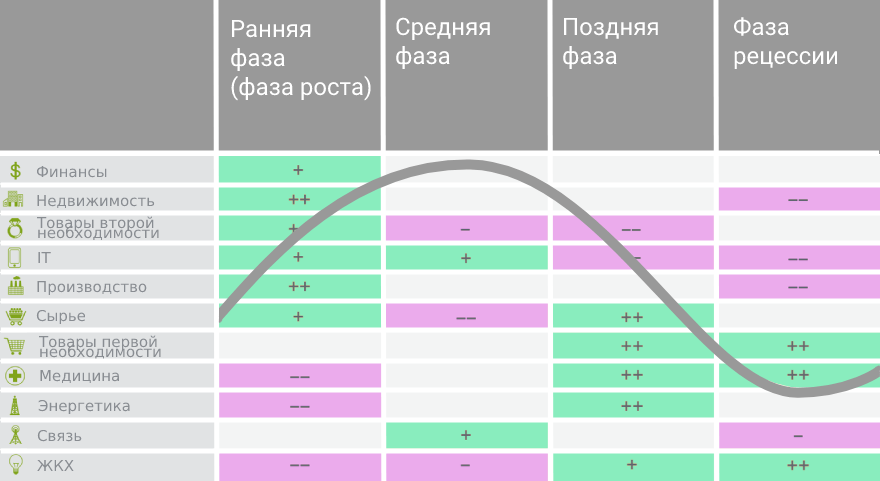
\includegraphics[scale = 0.47]{sectors_rus.jpg}
			\caption{Сектора в различных фазах экономики (\textit{источник: bcs-online.ru})}
			\label{model}
		\end{figure}
		
		Зная такие закономерности, вы можете предположить, что если мир подступает к рецессии, то лучше вкладываться в акции сектора здравоохранения. Если же дно пройдено и начинаются первые шаги к восстановлению, то выгоднее вкладываться в финансовый сектор и промышленный сектор. Эти закономерности довольно устойчивы, но основная сложность использования данной модели в том, чтобы точно определить, на какой стадии цикла находится экономика. Для рецессии существует точное определение (снижение ВВП в течение двух кварталов подряд), для других же стадий не существует строгих рамок.
		\newpage
		\item \textbf{Для того, чтобы точнее оценить результаты управления портфелем.} На рисунке ниже показан вклад в итоговую доходность, которую внесла каждая из индустрий.
		\begin{figure}[h]
			\centering
			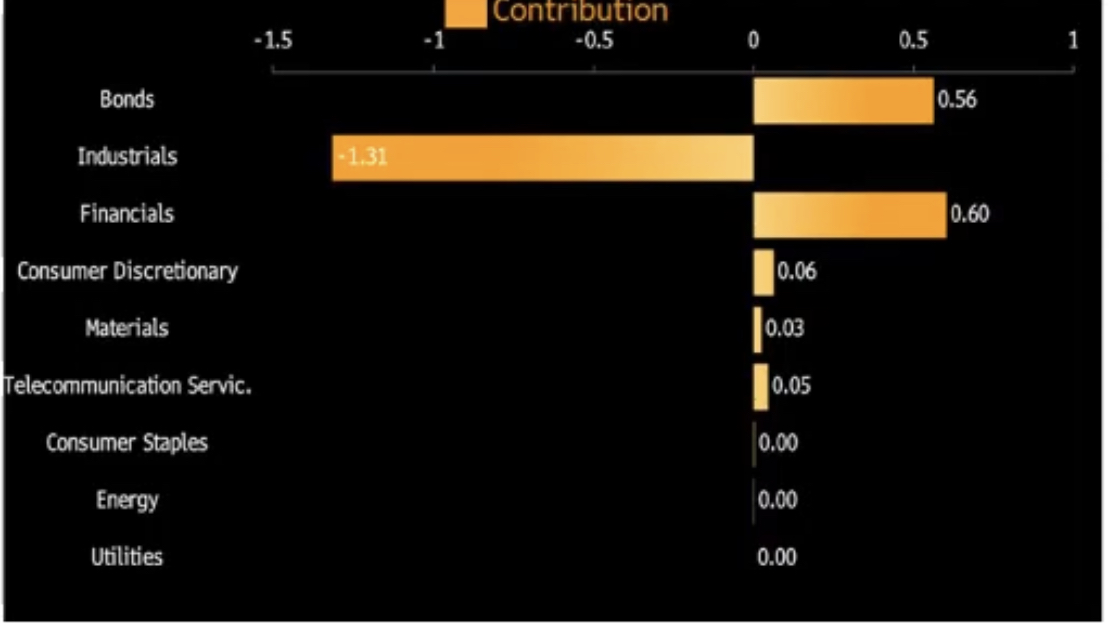
\includegraphics[scale =0.3]{example_port.jpg}
			\caption{Пример портфеля и доходность каждого сектора экономики}
			\label{model}
		\end{figure}
		
		Разобрав доходность портфеля по индустриям, мы можем точнее оценить, что было сделано правильно, а что неправильно, или если мы оцениваем внешнего менеджера, мы можем сделать вывод, давать ли ему денег в управление.
		
	\end{enumerate}
	
	
	
	\section{Как можно сгруппировать компании на сектора, подсектора индустрии?}
	\subsection{По каким принципам можно сгруппировать отрасли?}
	\begin{enumerate}
		\item \textbf{По основному направлению бизнеса компании.} Если мы имеем дело с сетью ресторанов, то основная выручка получается от изготовления и продажи еды, авиакомпании занимаются продажей билетов и перевозками. Для каждого такого направления деятельности можно выделить и найти свою группу компаний, которые являются определённой индустрией.
		
		\item \textbf{По чувствительности к стадии бизнес цикла.} Есть некоторые направления бизнеса, которые очень сильно зависят от настроения потребителей, от того, как себя чувствует экономика, и в то же время есть другая группа, например, сектор здравоохранения: люди болеют вне зависимости от того, на каком этапе находится экономический цикл, то есть цикл здравохранения не является сильно чувствительным к макроэкономическим параметрам и по этой причине иногда называется защитным.
	\begin{figure}[h!]
			\centering
			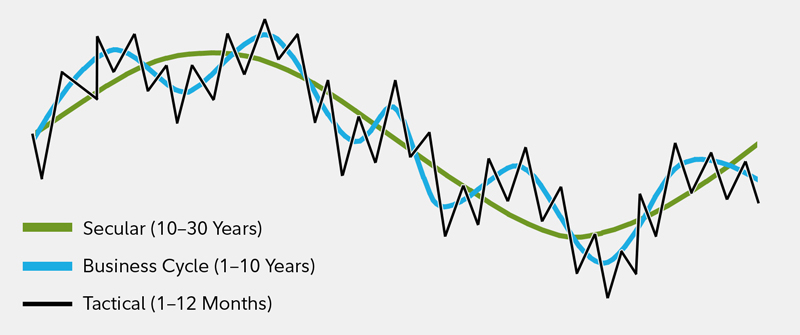
\includegraphics[scale = 0.38]{cycle1.jpg}
			\caption{Экономический цикл}
			\label{model}
		\end{figure}
		\newpage
		
		\begin{figure}[h]
			\centering
			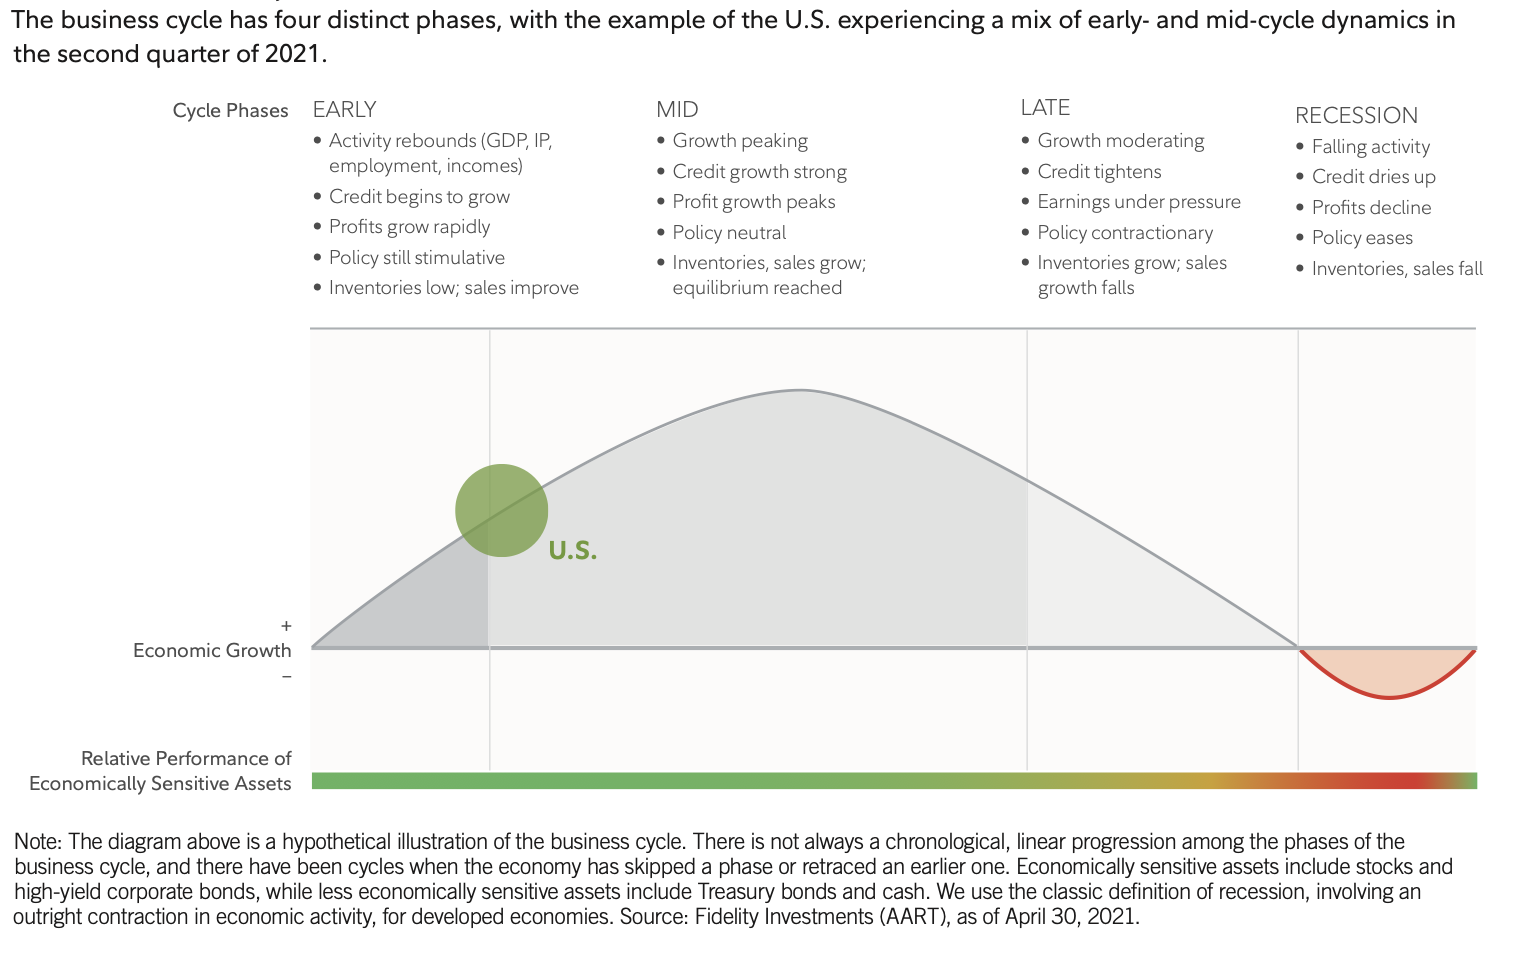
\includegraphics[scale = 0.64]{cycle2.png}
			\caption{Характеристика фаз экономических циклов (\textit{источник: fidelity.com})}
			\label{model}
		\end{figure}
		
		
		
		\item \textbf{По каким-то статистическим закономерностям.} Необязательно присутствие какой-то экономической логики, а можно, например, сгруппировать компании по волатильности акций, по размерам самих компаний или просто загрузить данные, с помощью методов машинного обучения автоматически найти какие-то закономерности и сгруппировать компании по каким-то определенным статистическим параметрам, которые мы и сами не могли придумать.
		
	\end{enumerate}
	
	\subsection{Системы классификации отраслей}
	
	В мире существуют тысячи компаний, у которых акции торгуются на биржах, из-за чего довольно затруднительно для каждой компании определить, к какому же сектору она относится, поэтому на помощь инвесторам приходят компании, которые составляют коммерческие классификаторы. Такие компании занимаются тем, что анализируют деятельность компаний и записывают компании в тот или иной сектор экономики, чтобы потом инвесторы, заплатив за доступ к такой базе данных, могли легко понять и сделать выводы о том, какие есть компании в определенном секторе.
	
	\textbf{Три самые распространенные коммерческие системы классификации:}
	\begin{itemize}
		\item GICS (Global Industry Classification Standard), или ГСКО (Глобальный стандарт классификации отраслей). В основном распространен в США.
		\item ICB (Industry Classification Benchmark), или Международный стандарт классификации. В основном используется в Европе.
		\item RGS (Russell Global Sectors), или Стандарт классификации от компании Расселл. Он используется очень редко.
	\end{itemize}
	
	
	Также существуют и \textbf{классификации, основанные на подсчетах, которые ведут гос. органы:}
	\begin{itemize}
		\item ISIC (The International Standard Industrial Classification of All Economic Activities), или МСОК (Международная стандартная классификация всех видов экономической деятельности).
		\item NAICS (The North American Industry Classification System), или Североамериканская система отраслевой классификации.
		\item Коды ОКВЭД (Общероссийский классификатор видов экономической деятельности).
	\end{itemize}
	
	Такие классификации не могут использовать инвесторы, так как органы статистики собирают информацию в агрегированном виде, то есть у них есть информация о том, куда, в какую группу, в какой сектор экономики относить каждую компанию, но в общем доступе находятся только агрегированные данные по отраслям, поэтому интересующую информацию по отдельным компаниям по таким классификаторам получить невозможно.
	
	\subsubsection{Система классификации GICS}
	
	Рассмотрим пример по системе классификации GICS.
	Эта классификация состоит из нескольких уровней, на первом уровне находятся 11 секторов экономики, на следующем уровне в каждом секторе находятся несколько индустрий, а индустрии подразделяются на подиндустрии. Всего существуют 4 уровня классификации. Рассмотрим первый уровень: он уже позволяет составить какое-то мнение о компании и ее особенностях.
	
	\underline{\textbf{Какие существуют сектора по стандарту GICS?}}
	\begin{itemize}
		
	\item \textbf{Consumer Discretionary} (потребительские товары, спрос на которые сильно зависит от стадии экономического цикла). Он называется так, потому что люди все время принимают решение, тратить на эти товары деньги или нет. Например: обувь, одежда, машина. Когда происходит спад, высокая безработица, зарплаты не растут, то люди, как правило, или тратят деньги на более дешевые товары, или вообще отказываются от дорогостоящих товаров.
	
	\item \textbf{Consumer Staples} (товары повседневного потребления, спрос на которые гораздо меньше зависит от состояния экономики). Сюда относятся товары повседневного потребления, например, продукты питания, средства гигиены, туалетная бумага и т.д.
	
	\item \textbf{Information Technology} (информационные технологии). Здесь всё, что касается развития технологий, например, если дальше разбить этот сектор на индустрии, то тут имеются 2 индустрии: Hardware (технологии, касающиеся железа) и Software (технологии, касающиеся программного обеспечения). Подиндустриями являются различные классы программного обеспечения и различные классы компьютерного оборудования.
	
	\item \textbf{Telecom} (связь). Сюда относятся компании, которые ведут деятельность по прокладке линий связи, по обеспечению услуг, например, это интернет-провайдеры, провайдеры сотовой связи, спутниковое телевидение и т.д.
	
	\item \textbf{Industrials} (промышленные компании). Здесь есть компании, которые производят какую-либо продукцию, которая затем используется другими корпорациями для производства чего-либо, например, для производства станков.
	
	\item \textbf{Materials} (материалы) - исходное сырьё для того, что используется в промышленности, например, ценные (золото и серебро) и неценные металлы (например, алюминий).
	
	\item \textbf{Energy}. Сектор связан с энергетикой, а именно: добычей, переработкой, транспортировкой нефти, газа и других источников энергии. Сектор делится на 3 индустрии: upstream (добыча), midstream (транспортировка) и downstream (переработка).
	
	\item \textbf{Financials} (финансовый сектор). Здесь находятся банковские компании, страховые компании, компании, управляющие активами и т.д.
	
	\item \textbf{Real estate}. Сектор связан с недвижимостью, появился несколько лет назад в данной классификации.
	
	\item \textbf{Utilities} (компании сферы ЖКХ). Компании из этого сектора занимаются генерацией, транспортировкой по сетям, водоотведением, канализацией, вывозом мусора и т.д.
	
	\item \textbf{Healthcare} (сектор здравоохранения). Сюда относятся фармацевтические компании, которые производят лекарственные препараты, частные больницы, поликлиники и т.д.
	\end{itemize}
	
	
	
	\subsubsection {Защитные и циклические сектора}
	\begin{itemize}
	\item \textbf{Компания из циклического сектора} - та, у которой прибыль сильно зависит от стадии бизнес цикла, то есть она подвержена настроениям потребителей и компаний. Например, при упаде в экономике отсутствует потребительский спрос, тогда, с одной стороны, люди не тратят деньги на покупку товаров, с другой стороны, компании, которые производят эти товары, у своих поставщиков заказы снижают из-за отсутствия потребительского спроса. Сюда относятся следующие секторы: энергетика, финансовый сектор, технологический, материалы и товары второй необходимости.
	
	\item \textbf{Компания из защитного сектора} - компания, чьи товары в гораздо меньшей степени зависят от экономического цикла. Сюда относятся следующие секторы: здравоохранение, ЖКХ и товары повседневного спроса.
	\end{itemize}

	\textit{Замечание 1.} При такой классификации всегда следует помнить, что это деление не является абсолютным. Стадии бизнес цикла не совпадают во всех странах (даже в пределах одной страны стадии бизнес цикла могут быть разными).
	
	 \textit{Замечание 2.}Всегда существуют компании, динамика которых в данный момент определяется именно факторами, присущими самой компании, а не стадиями экономического цикла в целом. Пример: Apple в 2008-2009 представила первый iPhone, который получил большую популярность, и компания очень сильно росла, несмотря на то, что по всей экономике наблюдался спад (у компании вышел удачный продукт, то есть такие события могут нарушать ход вещей).
	
	\textit{Замечание 3.} Защитные компании не означают, что если будет обвал, то их акции вырастут и не упадут, как правило, означают, что в таком случае их динамика будет более сглаженной. 
	
	
	\section{Peer group}
	
	\textbf{Peer group} - набор похожих компаний. Под похожими подразумевается, что они занимаются одинаковым бизнесом, спрос на их товары также определяется одними и теми же факторами, имеют схожую структуру издержек, схожую доступность капитала и географические регионы присутствия.

	Если мы просто ориентируемся на готовую классификацию, например, GICS, то действовать только на основании этого классификатора не совсем правильно. Например, и Сбербанк, и J.P. Morgan находятся в одном секторе, в одной индустрии, но у них и клиентская база, и регионы совершенно разные.
	Еще один пример: Google, Microsoft и Apple имеют пересекающиеся продукты, но если ориентироваться на готовый классификатор, то основной бизнес Google - интернет реклама, Microsoft - ее ОС и офисный пакет, а у Apple - продажа компьютеров и смартфонов. Несмотря на то, что эти компании конкурируют на некоторых рынках, говорить, что они непосредственно входят в такую peer группу, неправильно.
	
	\textbf{Шаги для верного составления набора сравнимых компаний:}
	\begin{enumerate}
		\item Использование коммерческой классификации, нахождение кандидата для дальнейшего подробного рассмотрения.
		\item Анализ финансовой отчетности интересующей нас компании на предмет упоминания конкурентов. Если компания является публичной, то она обязана опубликовать периодичную отчетность (по кварталам, по полугодиям и по годам). В годовом отчете есть определенные параграфы, которые компания обязана раскрывать, в том числе и конкуренцию в ее бизнесе.
		\item Анализ финансовых отчетностей компаний-конкурентов из предыдущего пункта.
		\item Использование специфических публикаций, специфической отраслевой аналитики, где можно найти информацию о последних трендах и сузить список peer компаний.
		\item Окончательный анализ оставшихся компаний, чтобы подтвердить, что они действительно схожи по оставшимся параметрам, которые не разобрали ранее (та же самая география или структура издержек).
		\item Скорректировать финансовую отчетность для того, чтобы составить сравнительные характеристики. Например, у компании будет отмечаться то, как они ведут отчетность, как они отражают те или иные особенности бизнеса в отчетности.
	\end{enumerate}
	
	
	\section {Важные элементы анализа индустрии}
	\begin{enumerate}
	\item Необходимо установить, какие макроэкономические перемены влияют на данную индустриию и какие тренды наблюдаются в соответствии с макроэкономическими переменами. 
	
	Это скриншот из информационно-аналитического терминала Bloomberg, где показаны переменные, влияющие на сектор индустрии авиаперевозок. 
	\begin{figure}[h]
		\centering
		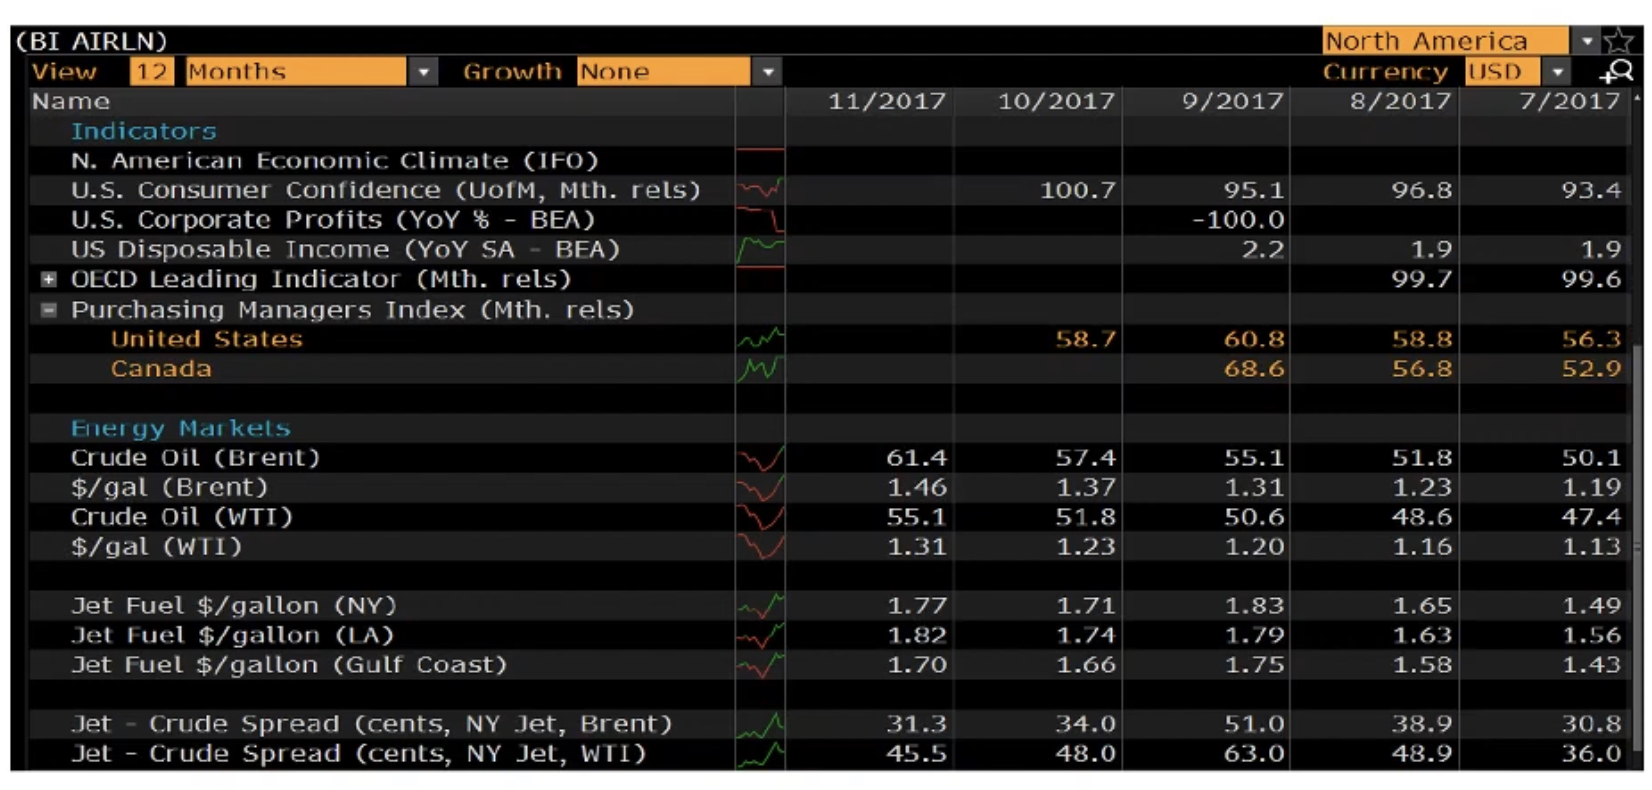
\includegraphics[scale = 0.25]{avia.jpg}
		\caption{Индикаторы, влияющие на сектор авиаперевозок (\textit{источник Bloomberg})}
		\label{model}
	\end{figure}
	
	Давно было установлено, что один из главных показателей, коррелирующих с объемом перевозок, - это темп роста ВВП. Если шагнуть ниже, то это, во-первых, такие индикаторы, как уверенность потребителей, темп роста прибыли корпораций. Авиаперевозками пользуются не только физ. лица, но и корпорации, которые отправляют сотрудников в командировку. Если увеличивается темп роста ВВП, то компании, скорее всего, расширяются и увеличивают объем покупок авиабилетов, чтобы устанавливать новые связи. С другой стороны, на бизнес авиакомпаний влияют издержки, и основная из них это, конечно, топливо, поэтому на скриншоте сразу показана динамика цен на нефть и авиатопливо.
	
	\item После установления взаимоотношений макроэкономики и индустрии надо составить несколько сценариев: базовый, негативный и оптимистичный. Затем надо посмотреть, что, в соответствии с нашими прогнозами, станет с сектором, который мы анализируем.
	
	\item Cравнить наши сценарии с тем, какие остальные аналитики дают прогнозы, или, иначе говоря, какой консенсус-прогноз по индустрии, по отдельным переменным, чего ожидает рынок в среднем.
	Ниже скриншот из Bloomberg, где показано мнение отдельных аналитиков из различных банков по цене на нефть Brent. 
	\begin{figure}[h]
		\centering
		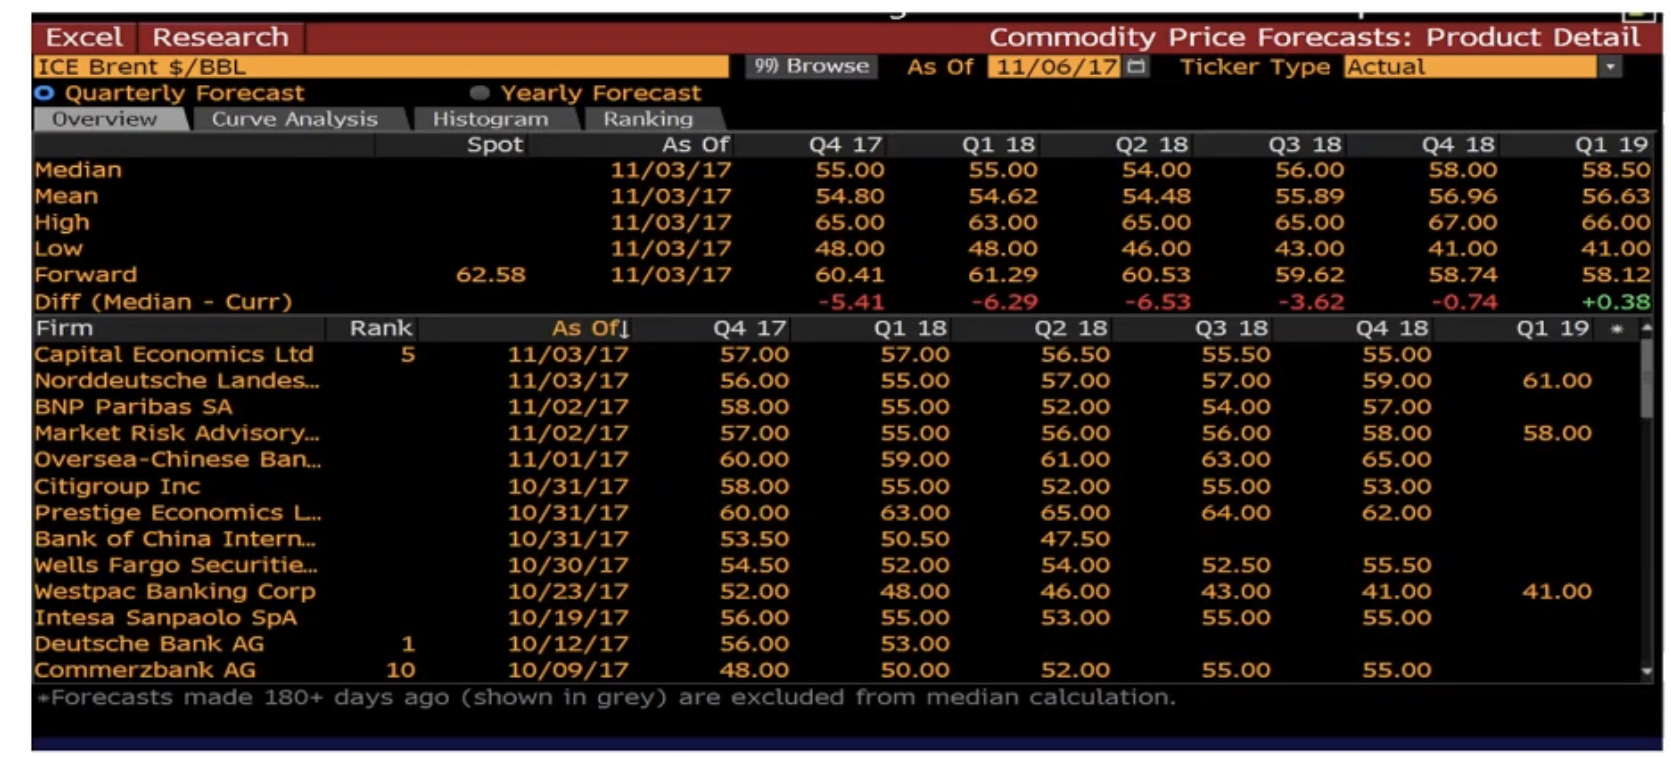
\includegraphics[scale = 0.25]{brent.jpg}
		\caption{Прогнозы аналитиков по цене на нефть Brent (\textit{источник Bloomberg})}
		\label{model}
	\end{figure}
	
	Установив мнения других участников рынка, мы можем составить представление о том, насколько наши прогнозы пессимистичны или оптимистичны. 
	
	\item Определение относительной оценки различных индустрий. Здесь речь идет о том, что может сложиться ситуация, когда соседние индустрии имеют различные оценки, отличающиеся в разы, то есть некоторые компании могут быть переоценены, могут быть недооценены, это надо обязательно отражать в анализе индустрий.
	
	\item Cравнение индустрии самой с собой, то есть насколько компании в этой индустрии стоят дороже или дешевле по отношению к ним же самим в прошлые периоды времени.
	
	\item Анализировать индустрию с точки зрения классификации на стратегические группы. Стратегические группы  - группы компаний, которые принадлежат одной индустрии, но очень сильно отличаются особенностями бизнеса. Например: в секторе авиаперевозок есть традиционные авиакомпании и авиакомпании-дискаунтеры, которые выставляют цену на билеты гораздо ниже, но зато берут деньги за допоолнительные услуги, где зарабатывают основную маржу. Что компания-дискаунтер, что традиционная авиакомпания занимаются одним и тем же бизнесом, и макроэкономические перемены влияют на них одинаково, но, с точки зрения анализа индустрии, они принадлежат к разным стратегическим группам.  Другой пример: фармацевтический сектор, в котором есть компании, которые большие деньги тратят на разработку новых лекарств, а есть компании, которые следят за истекающими патентами и выпускают аналоги уже других лекарств, которые сходны по формулам с препаратами, на которые уже истек патент.
	
	\item Определение, на какой стадии жизненного цикла находится компания.
	
	\item Посмотреть, каково соотношение издережек и выпуска. Иначе говоря, насколько важен эффект масштаба в той индустрии, которую мы анализируем.
	
	\item Исследовать внешние факторы, которые могут оказывать влияние и приводить к резким изменениям в индустрии. Например, это демографические факторы, вмешательство госудраства, социальные факторы или какие-то технологические сдвиги.
	
	\item Анализ степени конкуренции, которая сейчас наблюдается в индустрии. 
	
	\end{enumerate}
	
	\section{Анализ сил, оказывающих влияние на уровень конкуренции в данной индустрии}
	
	\textbf{5 сил Портера} - это 5 факторов, которые впервые были веделены Майклом Портером в его книге по стратегическому управлению компаний. Это была первая попытка разобрать процесс бизнеса не с точки зрения сил, направленных внутрь компании (издержки компании, как организованы рабочая сила, каналы сбыта и т.д.), а именно с точки зрения, что компания не существует в вакууме, а у нее есть внешняя среда, зачастую очень агрессивная, и у нее есть очень агрессивные конкуренты. Поэтому выстраивать стратегию компании и стратегию управления нужно с учетом вот таких сил, которые постоянно оказывают влияние на компанию и индустрию в целом.
	
	\textbf{5 сил Портера:}
	\begin{itemize}
	\item \textbf{Сложившийся уровень конкуренции между текущими участниками отрасли.} Чем выше конкуренция, чем чаще компании предпринимают шаги по изменению своих стратегий, чем чаще меняется лидер в этой отрасли, тем более конкурентная эта отрасль. Значит, скорее всего, чтобы заработать там какую-то прибыль, нужно прикладывать гораздо больше усилий и, скорее всего, результат не будет таким хорошим, как в индустрии, где уровень конкуренции низкий.
	\item \textbf{Угроза появления новых конкурентов.} Это связано с понятием барьеры входа (насколько просто начать новый бизнес, насколько легко может появиться новый конкурент). Например, открыть палатку с шаурмой просто, а создать нового автопроизводителя требует больше затрат и сил.
	\item \textbf{Угроза появления товаров-субститутов (заменителей).} Например, несколько лет назад были популярны цифровые камеры, но с развитием технологий камеры в мобильных телефонах стали настолько высокого качества, что большинство людей стало удовлетворяться и фотографиями, полученных с телефона. Тогда сегмент относительно дешевых цифровых видеокамер просто умер, и теперь остались или смартфоны, или дорогие зеркальные камеры. Поэтому опять же надо принимать во внимание то, насколько вероятно появление таких товаров-субститутов, которые могут быть даже родом не из нашей индустрии, а прийти из совершенно иной.
	\item \textbf{Переговорная сила покупателей.}
	\item \textbf{Переговорая сила поставщиков.}
	\end{itemize}
	Здесь надо помнить, что компания всегда обслуживает клиентов, а ее существование опирается на поставщиков. Если в этих отношениях наблюдается дисбаланс, то это может приводить к очень серьезным последствиям.
	Пример: несколько лет назад у компании Apple был поставщик защитных стекол для дисплея. Так как бизнес по производству iPhone рос, и Apple покупала постоянно эти защитные экраны только у данной компании, следовательно, и бизнес этой компании рос, как на дрожжах. В итоге, компания переориентировалась на Apple и стала ее основным поставщиком, а Apple стала ее основным клиентом, при этом Apple, пользуясь тем, что она единственный клиент, постоянно требовала снижения цен под предлогом того, что она может перейти к другому поставщику. Здесь и появляется переговорная сила покупателя. Эта компания по производству стёкол снижала цены на свои стёкла до очень низкого уровня. Когда после очередных переговоров компания сказала, что дальше не будет снижать свои цены, Apple сказала, что если так, то они отказываются продолжать сотрудничество и уходят к другому поставщику. Эта компания по производству стёкол просто обанкротилась. Точно так же это работает и в другую сторону. Если мы опираемся на маленькое количество поставщиков, с одной стороны, они тоже могут диктовать свои условия, с другой стороны, даже если непреднамеренно случится какой-то форс-мажор, нарушится цепочка, то мы тоже окажемся в невыгодном положении.
	
	
	\section{Факторы, влияющие на степень конкуренции}
	\begin{itemize}
		\item \textbf{Барьеры входа:} насколько легко новый участник может получить капитал, интеллектуальную собственность, клиентскую базу. Чем проще появление нового кокунрента, тем больше уровень конкуренции. Если из года в год лидерами в индустрии остаются одни и те же компании, значит, барьеры входа появления новых конкурентов довольно велики. Опять же может быть такое, что начать какой-то бизнес в какой-то отрасли не так сложно, например, создать новую марку одежды или новое кондитерское производство, но тем не менее в таких индустриях настолько велика сила бренда, что очень тяжело занять значимые позиции, поэтому когда говорят о барьерах на вход, то это необязательно означает сложность просто начать бизнес, здесь идет речь о том, чтобы этот бизнес взрастить и стать действительно успешным игроком. Барьеры могут меняться со временем. 
	
	\item \textbf{Уровень концентрации в индустрии:} всем известно, что если существует монополия, то она диктует свои цены и, соотвественно, для компаний это самый оптимальный вариант, но монополий почти ни в каких отраслях не наблюдается. Вообще Портер говорил, что существуют две основные стратегии для создания успешного бизнеса:
	\begin{enumerate}
	\item Оптимизация издержек.
	\item Продуктовая дифференциация. Мы делаем товар, который намного лучше, чем другие, или же у него есть другие качества, которые позволяют нам диктовать цены и устанавливать цены выше, чем другие компании.
	\end{enumerate}
	% пример такого подхода: apple vs apples (существует куча хозяйств , которые выращиюват яблоки и продают яблоки +- по одной цене, они отличаются сортами, но можно купить яблоки в любом магазине. в противовес, маркетинговая стратегия эппл, которая создала образ особенной комании, в итоге, ее смартфоны (хоть они и по функциональности сравнимы с остальными) стоят в среднем гораздо дороже, чем смартфоны других фирм  просто за счет четко выстроенной маркентиговой стратегии. в резульатте,  в отрасли производства смартфонов сложиласьтакая ситуация:  существуют 2 лидера с смаыми большими рыночнымидолями  эппл и самсунг, существубт несколько компаний поменьше, котоыре нашли свою нишу и реализуют  стратегию производства более дешевых смартфонов (хуавей и сяоми) и есть огромное количество всех остлаьных участинков рынка, доли которых настолько млаы, что их в статистике показывают строчкой "прочее",между ними и разгарается основная  борьба . таким образом, чем больше уровень концентрации в индустрии, чем более она похожа на монополию или олигаполию, тем большую маржу она может зарабатывать, то есть более высокие цены ставить 
	
	\item \textbf {Максимально возможный объем производственных мощностей в данной индустрии}. Он влияет на цены и доходность инвестиций. Аналитик должен иметь представление о текущем потенциале отрасли. Рассмотрим на примере: несколько лет назад из-за долгосрочного роста спроса на нефть вырос и спрос на перевозки нефти. Так как до этого долгое время спрос на перевозки не рос особо, то флот танкеров не расширялся. Когда спрос вырос, а флот танкеров остался тем же, цены на перевозки нефти на танкерах очень сильно выросли. В результате, компании, владеющие этими флотами, решили расширять флот и заказали большое количество новых танкеров. Постройка танкеров занимает больше года, к тому времени, когда были готовы новые танкеры, структура спроса и предложения уже изменилась, а флот танкеров увеличился, уже не нужен был такой обьем. Тогда цены на перевозки драматично упали, и компании с флотами танкеров обанкротились. Очень важно следить, каков максимально возможный объем производственных мощностей, как близко к пределу находится текущее состояние и как это может повлиять на всех участников рынка. 
	
	\item \textbf{Стабильность долей рынка отдельных участников.} Сильно варьирующиеся доли рынка означают высоко конкурентную индустрию. Если просмотреть хронологию и увидеть, что из года в год лидер в отрасли меняется, то это типичный показатель того, что отрасль является высоко конкурентной, и высокой прибыльности от этих компаний в этой отрасли можно не ожидать.
	
	\end{itemize}
	\newpage
	
	\section{Модель жизненного цикла индустрии}
	
	\begin{figure}[h]
		\centering
		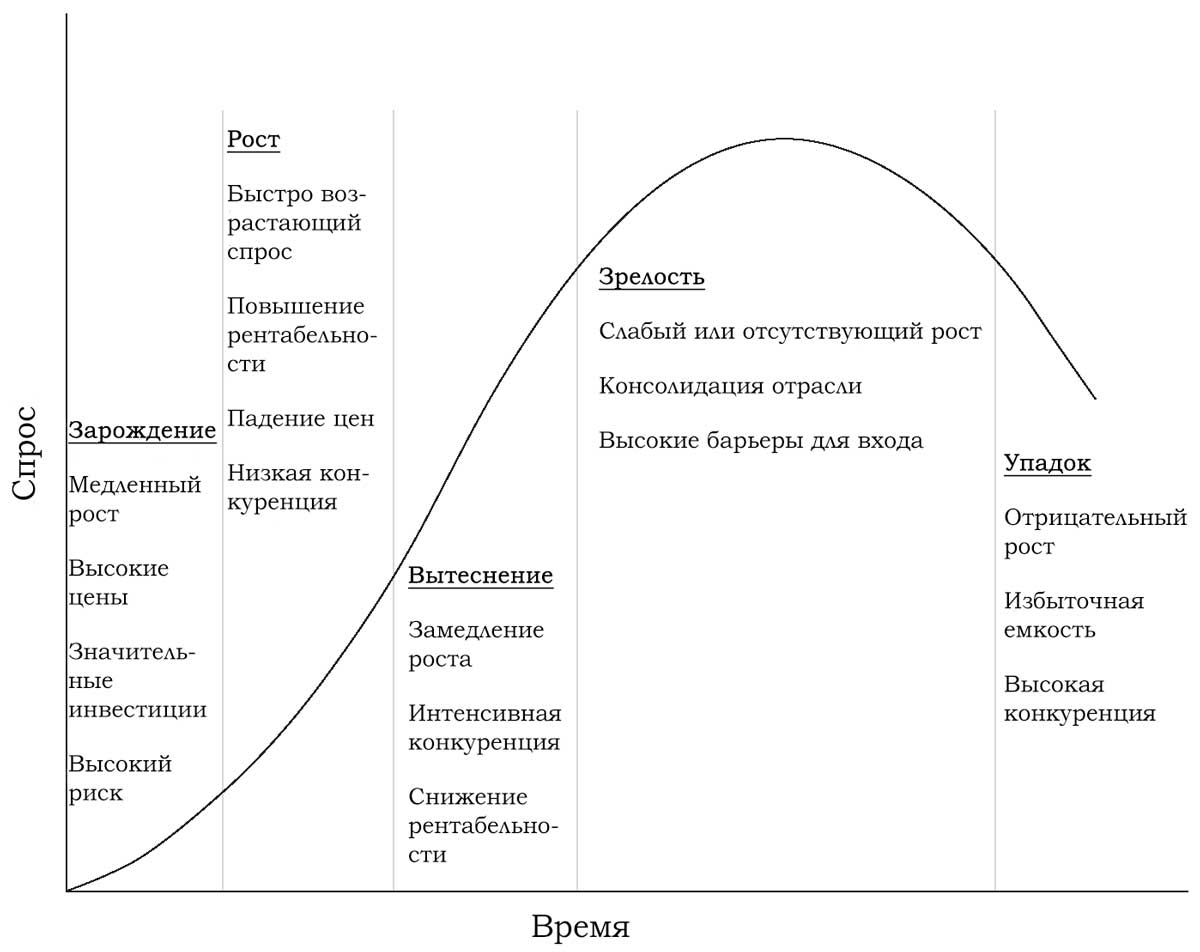
\includegraphics[scale = 0.35]{life_cycle_industry.jpg}
		\caption{Жизненный цикл индустрии}
		\label{model}
	\end{figure}
	Для того, чтобы охарактеризовать ту или иную индустрию, используют модель жизненного цикла индустрии. 
	Эта модель говорит, что каждая индустрия проходит несколько этапов развития. Таким образом, определив, на каком из этапов развития находится данная индустрия, мы можем сделать определенные выводы о том, какие процессы в ней сейчас происходят, с какой скоростью и чего ждать в дальнейшем.
	
	\textbf{Стадии жизненного цикла:}
	\begin{enumerate}
		
	\item \textbf{Стадия эмбриона.} Появляется какая-то новая идея, новый продукт, вокруг которого в дальнейшем начинает формироваться целая индустрия, то есть набор компаний, которые занимаются развитием этого продукта. Когда продукт только появляется, то тут идет речь о маленьких масштабах, продукт очень дорогой, очень мало энтузиастов им интересуются, поэтому рост индустрии ограничен, к тому же она требует больших инвестиций и риски высоки. Как правило, в такие компании и индустрии инвестируют венчурные инвесторы. Компании на этой стадии не представлены на бирже и не являются публичными. 
	\item \textbf{Стадия роста.} Если идея или продукт действительно успешны, то это означает, что большее количетво людей начинает интересоваться. Благодаря эффекту масштаба можно экономить на издержках и снизить цены, в результате рост ускоряется, увеличивается количество людей, знакомых с продуктом и интересующихся им. По-прежнему уровень конкуренции ограничен, так как очень мало компаний занимались этой идеей, развивали ее и вкладывали в нее. Вначале наблюдается несколько лидеров, которые растут очень быстрыми темпами, и, снижая издержки, они зарабатывают.
	\item \textbf{Стадия встряски/вытеснения.} Если же в течение некоторого периода идея продолжает показывать очень хорошую прибыль, то наблюдается следующая стадия shake out (встряска), когда в эту индустрию приходят новые игроки, обладающие большим капиталом, тогда уровень конкуренции очень сильно увеличивается, компании инвестируют в расширение, как правило, это приводит к замедлению роста, и приходим к положению overcapacity (когда уровень доступных производственных мощностей опережает необходимые для удовлетворения спроса). Это означает, что компании начинают пытаться хоть как-то продать свой продукт, с одной стороны, им нужно увеличивать рекламный бюджет и бороться с конкурентами, с другой стороны, им нужно снижать цены, в результате это приводит к снижению прибыльности.
	\item \textbf{Стадия зрелости.} Наблюдается консолидация, то есть с рынка уходят слабые убыточные игроки, и остается несколько крупных компаний, которые продолжают сохранять уверенные позиции и не пускают  новых конкурентов. Таким образом, выстраиваются высокие барьеры на вход, а так как уровень конкуренции замедляется, то и цены становятся стабильными.
	\item \textbf{Стадия упадка.} Если продукт выходит из моды или становится ненужным, то наблюдается спад, цены продолжают падение, и иногда индустрию можно спасти тем, что оставшиеся игроки пытаются дополнительно консолидироваться и дополнительно экономить на издержках, что иногда приводит и к полному исчезновению индустрии. 
	\end{enumerate}

	Человек в своем развитии не может перескочить из одной стадии резко на другую или вернуться назад, при этом модель жизненного цикла для индустрии предусматривает такие скачки и возвраты. 
	\textbf{Что может привести к скачкам и возвратам?}
	\begin{itemize}
		\item \textbf{Технологические изменения.}
		\item \textbf{Изменения в регуляторной среде.} Например, индустрия по производству сыра в России до 2014 года была никому не нужной с маленькими объемами производства. Тем не менее после введения санкций и контрсанкций в 2014 году и запрета на ввоз множества продуктов индустрия по производству сыра в России вернулась на несколько стадий назад и пришла к экспоненциальному росту.
		\item \textbf{Социальные факторы.} Пример: ресторанный бизнес. На протяжении целых столетий ресторанами пользовались только очень обеспеченные люди, или же их использовали как место для отмечания каких-то праздников. Можно было сказать, что эта индустрия находилась примерно на стадии зрелости, но в начале 20 века после серьезных социальных преобразований женщины во многих странах в гораздо больших объемах стали включаться в рабочую силу, значит, у них стало гораздо меньше времени на то, чтобы готовить дома, помимо этого, бюджет семьи возрос, поэтому  в средней семье появились деньги, чтообы их потратить в кафе или ресторане. Так, рестораны из стадии зрелости перескочили на более ранние этапы.
		\item \textbf{Демографические факторы.} Например, целые индустрии производства товаров для детей или производства препаратов для пожилых людей зависят от того, какая сложилась демографическая обстановка в том или ином регионе. Если родилось большое количество детей, их нужно одевать, кормить, развлекать и т.д., поэтому спрос из-за этого демографического фактора может увеличиться в разы.
		\item \textbf{Внутри одной индустрии могут быть совершенно разные компании, показывающие разную динамику.} Например, в секторе производства смартфонов после 2008 года бывший лидер Nokia стал резко терять позиции, а новая компания Apple росла опережающими темпами по сравнению со всей отраслью. Таким образом, не все компании будут обладать одинаковыми характеристиками.
	\end{itemize}
	
	
	\section{От теории к практике}
	Давайте сравним 3 индустрии: авиалинии, сети супермаркетов и производители luxury товаров.
	\begin{figure}[h]
		\centering
		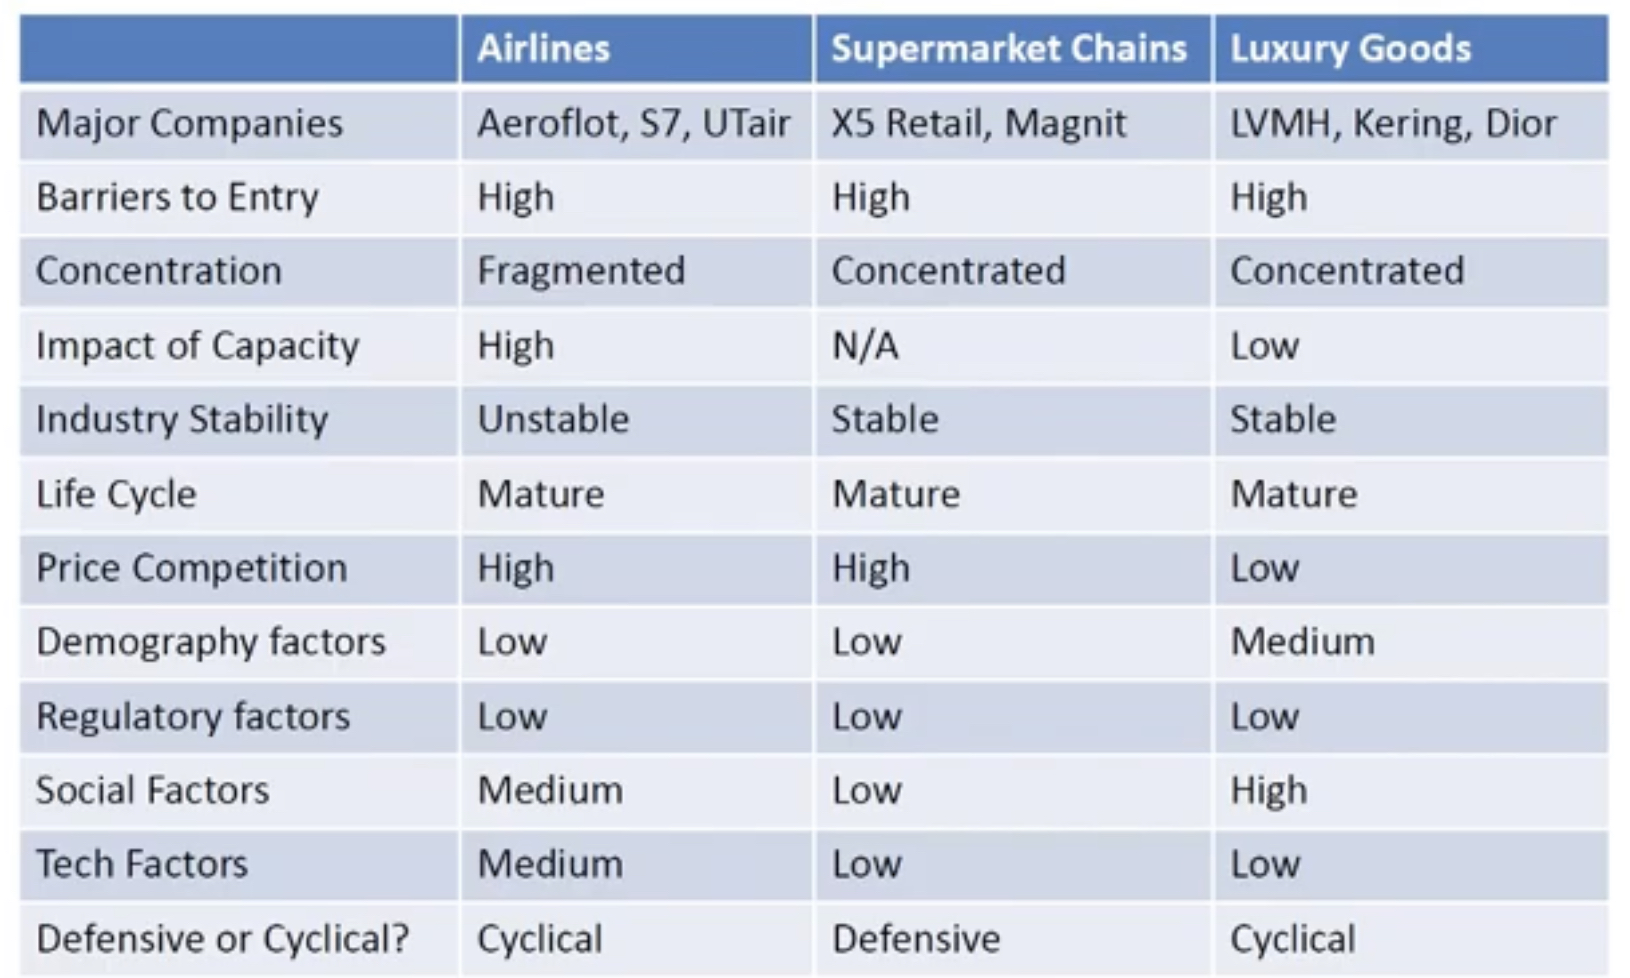
\includegraphics[scale = 0.27]{practice.jpg}
		\caption{Жизненный цикл индустрии}
		\label{model}
	\end{figure}

	\begin{itemize}
		\item \textbf{Барьер на вход.} Для авиалиний он высокий, так как даже если не покупать новые самолеты, а брать их в лизинг, то лизинговые платежи все равно составят огромный объем средств. Именно с точки зрения финансов это очень затратное мероприятие, не говоря уже о найме персонала. Для сетей супермаркетов барьер на вход высокий, так как не так дорого создать 1-2 магазина, но создать федеральную сеть, работающую по всей России, охватывающую основные города, - уже затраты совсем другого порядка. Для сферы luxury товаров барьер довольно высок, так как не так дорого создать производство, запустить линию по производству одежды, но достичь мирового масштаба и укрепить бренд - задача совсем другого уровня и совсем других затрат.
	
	\item \textbf{Концентрация в индустрии.} Авиалинии - это фрагментированная отрасль, так как если смотреть в целом, то люди выбирают того авиаперевозчика, который на интересующий их рейс установит самую низкую плату за билет. При этом, если говорить о супермаркетах и luxury товарах, это очень концентрированные отрасли с очень маленьким числом основных игроков. В сфере luxury существует большое количество разных брендов, но, на самом деле, они входят в малочисленные холдинги.
	
	\item \textbf{Влияние объема производственных мощностей.} Для авиалиний это влияние велико, потому что спрос может меняться очень быстро, а парк самолетов невозможно увеличить в течение нескольких дней или месяцев. С другой стороны, если спрос резко падает, то нельзя просто избавиться от лишних освободившихся самолетов. Для супермаркетов это не совсем правильный фактор, потому что здесь играет роль уровень производственных мощностей производителей товаров, которые представлены на полках супермаркетов, сами супермаркеты просто посредники. Для luxury товаров это влияние низкое, так как затраты на увеличение объема производства или его сокращение не так велики, в основном, они касаются рабочей силы.
	
	\item \textbf {Стабильность рыночных долей.} В авиалиниях эти доли нестабильны, потому что очень высока конкуренция за счет цен на билеты. Для супермаркетов и товаров luxury эти доли стабильны из-за того, что индустрия очень концентрированная.
	
	\item \textbf{Этапы жизненного цикла.} Все эти индустрии в стадии зрелости, так как никакого экспоненциального роста в этих отраслях нет, все они связаны с такими отраслями, которые уже на протяжении многих десятилетий существуют, развиваются, и пока что реальных изменений не очень видно.
	
	\item \textbf{Уровень конкуренции по ценам.} Для авиалиний высок вклад этого фактора, потому что цена на билет - один из основных факторов принятия решения о его покупке. Аналогично, это важный фактор для супермаркетов: чем дешевле товар, тем больше объем, тем больше людей будут покупать и интересоваться этим. Для luxury товаров этот фактор низок, потому что цена на эти товары иногда работает в обратную сторону: чем дороже товар, тем с большим удовольствием люди покупают его.
	
	\item \textbf{Фактор демографии.} Для авиалиний и супермаркетов не так важен, а для luxury товаров он более менее важен, потому что спрос на такие товары среди подростков и детей и среди пожилого населения гораздо меньше, чем среди людей среднего возраста.
	
	\item \textbf{Факторы государственного вмешательства и регулирования.} Во всех отраслях вклад этих факторов не так велик, строгих законов и ограничений здесь не наблюдается.
	
	\item \textbf {Социальные факторы.} Для авиалиний довольно среднее влияние, оно больше связано с представлениями людей о том, как они должны проводить свой отпуск, как они должны отдыхать, должны ли они летать, а также это фактор бизнес перевозок, командировок, бизнес-встреч. Для супермаркетов социальные факторы не играют большую роль, а для товаров luxury эти факторы играют большую роль, потому что эта отрасль зависит от моды, а мода имеет свойство быстро меняться.
	
	\item \textbf{Технологические факторы.} Для авиалиний их влияние на авиалинии среднее, в основном, оно касается улучшений именно в технологиях авиаперевозок, например, появление более экономичных двигателей, более вместительных самолетов и т.д. Для супермаркетов и сегмента luxury вклад технологий не так велик.
	
	\item \textbf{Тип отраслей.} Авиалинии - циклический бизнес, так как он напрямую связан с настроениями потребителей и бизнеса. Супермаркеты - защитная отрасль, так как в них, в основном, продаются товары повседневного спроса. Luxury товары - циклическая отрасль, потому что объемы таких покупок зависят от настроения потребителей, хороша ли ситуация в экономике.
	
	\end{itemize}
	
	\section{Группы факторов, влияющих на анализ индустрии в целом}
	\begin{itemize}
		\item \textbf{Макроэкономические факторы:} тренды по темпам роста ВВП, динамика процентных ставок в экономике, темпы инфляции.
	\item \textbf{Технологические факторы:} введение новых и улучшенных продуктов, снижение барьеров входа.
	\item \textbf{Демографические факторы:} в зависимости от состава населения, те или иные индустрии будут развиваться быстрее или медленнее.
	\item \textbf{Фактор государственного вмешательства:} реализовывается через изменение фискальной политики, уровня налогов, регулятивных мер или с помощью гос. закупок.
	\item \textbf{Социальные факторы:} анализ того, как люди работают, отдыхают, тратят деньги и т.д.
		\end{itemize}
	
	
	\section{Основные моменты в анализе компании и оценке ее акций}
	\begin{enumerate}
		\item \textbf{Обзор самой компании:} в чем состоит ее бизнес, как устроена ее производственная цепочка, в чем ее сильные и слабые стороны.
		\item \textbf{Характеристика индустрии:} описание индустрии и всех факторов, оказывающих влияние на компании, действующих в этой индустрии.
		\item \textbf{Факторы спроса на товары компании.}
		\item \textbf{Факторы издержек и производства.}
		\item \textbf{Применение стратегического подхода:} посмотреть уровень конкуренции в компании, то, какую стратегию она использует, насколько стабильно ценообразование в этой компании.
		\item \textbf{Проведя качественный анализ, можем переходить к количественному:} анализировать финансовую отчетность, составить мультипликаторы, по ним сравнить компанию с другими (нужны именно сравнимые компании) или с её историческими показателями в прошлом.
		\item \textbf{Составление прогноза:} прогноз финансовой отчетности, финансовых показателей в будущем и оценка справделивой стоимости компании в будущем.
	\end{enumerate}
	
	\textbf{Дополнительные обязательные пункты:}
	\begin{itemize}
		\item Обзор товаров и услуг, которые предоставляет компания.
		\item Анализ финансового состояния.
		\item Анализ стратегии компании.
	\end{itemize}
	

\end{document}

